\section{Theorie}
\label{sec:Theorie}

Schall ist ein physikalisches Phänomen, das Jedem bekannt sein sollte. 
Über Schall ist der Mensch in der Lage zu hören.
Dabei ist Schall eine longitudinale (in Festkörpern auch transversale) Welle die durch Druckschwankungen in einem Medium charakterisiert wird.
Die Frequenz dieser Welle bestimmt die Tonhöhe von dem was wir hören.
Allerdings ist der Mensch nur in der Lage Frequenzen von etwa $\SI{16}{\hertz}$ bis $\SI{20}{\kilo\hertz}$ zu hören.
Schall mit einer Frequenz im Bereich von etwa $\SI{20}{\kilo\hertz}$ bis $\SI{1}{\giga\hertz}$ wird Ultraschall genannt. \cite{US1}

Dieser Ultraschall kann dazu genutzt werden Materialien zu untersuchen, ohne dabei dieses Material zerstören zu müssen.
Wie diese Untersuchung funktioniert soll im Folgenden dargelegt werden.


\subsection{Beschreibung von Schall}
\label{ssec:theorie_beschreibung}

Da Schall eine Druckwelle ist, kann dieser über
\begin{equation}
    p(x,t) = p_0 + v_0 Z \cos(\omega t - k x)
    \label{eq:schallwelle}
\end{equation}
beschrieben werden. 
Eine wichtige Größe bei dieser Beschreibung ist die akustische Impedanz $Z=c \cdot \rho$.
Diese kann als eine Art Widerstand des Mediums betrachtet werden.
Er setzt sich zusammen aus der Schallgeschwindigkeit $c$ des Mediums und der Dichte $\rho$ des Mediums.

Da die Schallwelle beim traversieren des Mediums durch Absorption Energie verliert, nimmt die Intensität $I_0$ dieser exponentiell nach
\begin{equation}
    I(x) = I_0 e^{-\alpha x}
    \label{eq:absorption}
\end{equation}
mit der Strecke $x$ ab. 
Hier beschreibt $\alpha$ den Absorptionskoeffizienten der Schallamplitude.
Da bei Ultraschall in Luft $\alpha$ sehr groß ist, wird in der Regel der Schallerzeuger und das zu untersuchendem Medium über eine Flüssigkeit mit geringerem $\alpha$ gekoppelt.

An einer Grenzfläche zwischen zwei Medien wird der Schall teilweise reflektiert.
Dieses Verhalten kann über den Reflexionskoeffizienten
\begin{equation}
    R = \frac{I_\text{reflektiert}}{I_\text{einfallend}} = \left( \frac{Z_1 - Z_2}{Z_1 + Z_2} \right)^2
    \label{eq:refelxion}
\end{equation}
beschrieben werden.
Der Transmissionskoeffizient ist dann
\begin{equation}
    T = \frac{I_\text{transmittiert}}{I_\text{einfallend}} = 1 - R \, .
    \label{eq:transmission}
\end{equation}


\subsection{Anwendung von Ultraschall}
\label{ssec:theorie_anwendung}

Wie schon einleitend geschrieben kann mit Ultraschall ein Körper auf Fehlstellen bzw. örtliche Änderung des Materials untersucht werden.
Am bekanntesten ist hierbei die Ultraschallsonographie, die zur medizinischen Untersuchung schwangerer Frauen verwendet wird.

Dabei gibt es in der Laufzeitmessung von Ultraschall zwei verschiedene Verfahren:

\begin{figure}
    \centering
    \begin{subfigure}{0.3\textwidth}
        \centering
        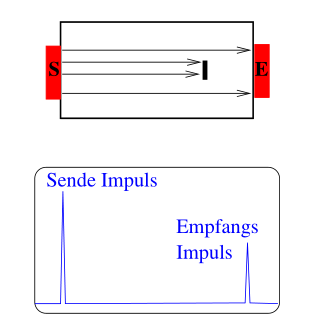
\includegraphics[width=\textwidth]{images/bild01.png}
        \caption{Durchschallungsverfahren}
        \label{fig:durchschallung}
    \end{subfigure}
    \begin{subfigure}{0.3\textwidth}
        \centering
        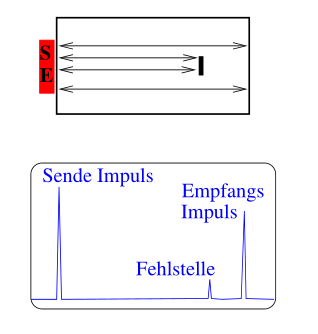
\includegraphics[width=\textwidth]{images/bild02.png}
        \caption{Impuls-Echo-Verfahren}
        \label{fig:impuls-echo}
    \end{subfigure}
    \caption{Die verschiedenen Verfahren der Laufzeitmessung eines Ultraschallimpulses mit entsprechendem A-Scan.\cite{US1}}
    \label{fig:verfahren}
\end{figure}

Zum Einen gibt es das Durchschallungsverfahren (siehe \autoref{fig:durchschallung}) in dem der Schallimpuls durch das Medium geschickt wird und auf der anderen Seite gemessen wird.
Hier wird die Intensität bei einer gefundenen Fehlstelle abgeschwächt. 
Allerdings kann keine genaue Aussage über die Position der Fehlstelle getroffen werden.

Zum Anderen gibt es das Impuls-Echo-Verfahren (siehe \autoref{fig:impuls-echo}) bei dem der Sender des Schallimpulses gleichzeitig auch als Empfänger dient.
Hier wird also die Reflexion an einer Grenzfläche ausgenutzt und der Reflektierte Impuls gemessen.
Hier kann über die Laufzeit des Impulses eine Aussage über die Lage der Fehlstelle getroffen werdem.
Die zurückgelegte Strecke des Impulses bis er reflektiert wurde kann über
\begin{equation}
    s = \frac{1}{2} c \cdot t
    \label{eq:strecke}
\end{equation}
berechnet werden.

Bei beiden Verfahren kann aus dem Intensitätsverhältnis des ausgesendeten und empfangenen Impulses die Größe der Fehlstelle abgeschätzt werden.
Die Intensitätsmessung kann auf verschiedene Arten visuell dargestellt werden. 

\begin{figure}
    \centering
    \begin{subfigure}{0.3\textwidth}
        \centering
        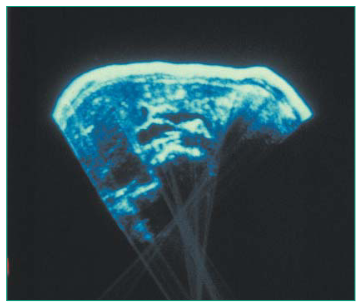
\includegraphics[width=\textwidth]{images/b-scan.png}
        \caption{B-Scan eines Oberbauchs}
        \label{fig:b-scan}
    \end{subfigure}
    \begin{subfigure}{0.5\textwidth}
        \centering
        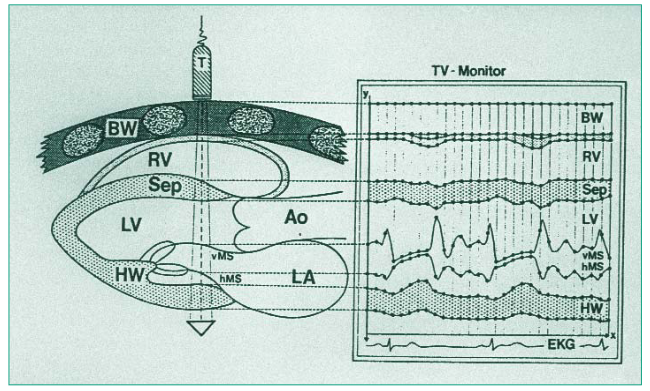
\includegraphics[width=\textwidth]{images/tm-scan.png}
        \caption{schematischer TM-Scan eines Herzen}
        \label{fig:tm-scan}
    \end{subfigure}
    \caption{Visualisierung der Scanverfahren.\cite{ultraschall-scans} (für den A-Scan siehe \autoref{fig:verfahren})}
    \label{fig:scans}
\end{figure}

Erstens gibt es den sogenannten A-Scan oder auch Amplituden-Scan, der die Schallamplitude in Abhängigkeit der Zeit in einem Diagramm darstellt. (siehe \autoref{fig:verfahren})

Zweitens gibt es den B-Scan oder auch Helligkeits-Scan, der die Schallamplitude in Abhängigkeit des Ortes in einem 2D-Bild darstellt, in dem die Helligkeit die Höhe der Schallamplitude darstellt. (siehe \autoref{fig:b-scan})

Und drittens gibt es den TM-Scan oder auch Time-Motion-Scan, der die Bewegung des zu untersuchenden Körpers darstellt, indem die räumliche Veränderung der Bereiche gleicher Impulsamplitude dargestellt wird. (siehe \autoref{fig:tm-scan})


Wie kann nun der Schallimpuls erzeugt bzw. gemessen werden?

Dazu wird häufig ein sogenannter piezoelektrischer Kristall verwendet.
Dieser kontrahiert bzw. expandiert wenn an diesen ein elektrisches Feldangelegt wird und erzeugt andersherum ein elektrisches Feld wenn dessen Volumen durch äußere Kräfte verändert wird.
Da dieser Effekt sehr schnell ist kann hiermit Ultraschall erzeugt werden.
Allerdings wird nur eine hohe Schallintensität durch die Schwingung dieses Kristalls erzeugt, wenn die Frequenz der Anregung nahe der Resonanzfrequenz des Kristalls ist.
Also werden für unterschiedliche Schallfrequenzen meist auch unterschiedliche Kristalle verwendet.

